\documentclass[../SMLreport_template.tex]{subfiles}
 
\begin{document}
Statistical machine learning algorithms tries to solve some form of task by attempting to predict an output variable, \textit{y} given some input vector, \textbf{\textit{x}}. This process can be described as function estimation. If a function, \(y = f(\textbf{\textit{x}}) + \epsilon\) exists that maps the input vector, \textbf{\textit{x}} onto the output, \textit{y}, with \(\epsilon\) representing the irreducible error, a statistical machine learning algorithm will approximate \(f\), with a model or estimate, \(\hat{f}\). Taking the frequentest perspective on statistics it can be assumed that the true model \(f\) is fixed but unknown while the estimate, \(\hat{f}\) is a function of the training data-set and can be described as a point estimate of f. Therefore, treating \(\hat{f}\) as a point estimator, its performance in estimating \(f\) can measured in terms of bias and variance errors. \par
\noindent 

The bias of an estimator is defined as \(bias(\hat{f}_n) = \mathbb{E}[\hat{f}_n] - f  \) where, \(\hat{f}_n\) is the point estimator obtained from the training dataset, \(\{\textbf{\textit{x}}_1, ... , \textbf{\textit{x}}_n\}\). It can be described as a measure of the expected deviation of the point estimator from the true model. It is a measure of how accurate the predictions of the machine learning model are. The variance of an estimator is defined as \(var(\hat{f}_n) = \mathbb{E}[\hat{f}_n^2] - \mathbb{E}[\hat{f}_n]^2 \) and is a measure of how the estimator varies as a consequence of the random data samples present in the training dataset. It is a measure of how precise the predictions of the machine learning model are. The effects of bias and variance are visualised in Figure \ref{acc} \par \noindent

\begin{figure}[t]
    \centering
    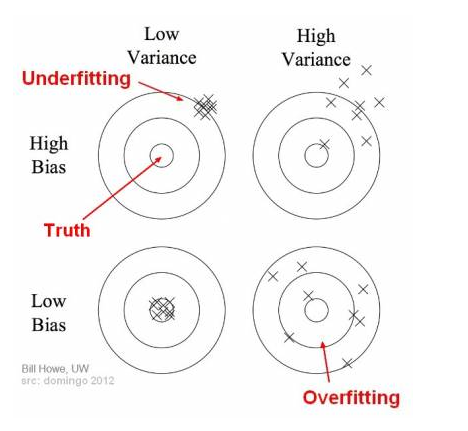
\includegraphics[width=0.5\textwidth]{images/accuracy.png}
    \caption{Visualisation of Bias and Variance}
    \label{acc}
\end{figure}

A defining characteristic of machine learning models is their ability to generalise to previously unseen input data. The generality of a machine learning model is tightly correlated to the relationship between the bias and variance of the estimator, \(\hat{f}\) which in turn are linked to the machine learning concepts of model complexity, underfitting and overfitting as shown in Figure \ref{bias_var}. Simple models tend underfit to the training dataset and struggle to memorise complex representations resulting in a high bias (poor model accuracy). Increasing the complexity of the models tends to decrease the bias of the model at the cost of variance with the model overfitting to the training dataset, learning complex representations that are only present in the training set, reducing the generality of the model. Therefore, the bias-variance trade off summarizes the fundamental tension in machine learning between model complexity and model generality as shown in Figure \ref{cap} and underlines the challenge in designing an estimator with the appropriate complexity \cite{goodfellow-bengio-courville}\cite{mehta-wang-Day-Richardson}. 

\begin{figure}[t]
    \centering
    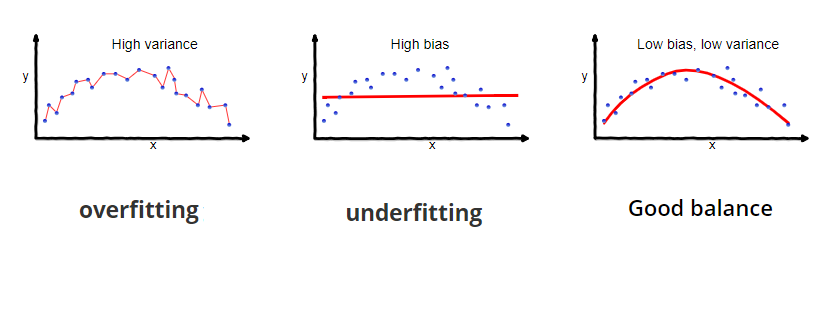
\includegraphics[width=0.5\textwidth]{images/model_fitting.png}
    \caption{Correlating Over and Under-fitting to Bias and Variance}
    \label{bias_var}
\end{figure}
\newpage

\begin{figure}[t]
    \centering
    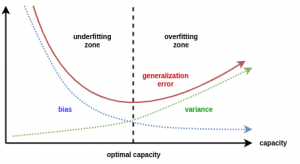
\includegraphics[width=0.5\textwidth]{images/capacity.png}
    \caption{The Fundamental Tension between Model Complexity and Model Generality}
    \label{cap}
\end{figure}



\end{document}